\section{Notions pr\'eliminaires}
\todomsg{quick sentence: first automata, then cache coherence}

\subsection{Automates temporis\'es}
\todomsg{quick sentence: first classical automata, then timed ones}
\subsubsection{Automates Classiques}

\begin{definition}[Classical Automata System]
A classical automata system \automatasystem{} is a
$\langle \automatastates{}, \allowbreak{}
\automatainit{}, \allowbreak{}
\automatacondlabels{}, \allowbreak{}
\automatachanlabels{}, \allowbreak{}
\automatavariables{}, \allowbreak{}
\automataactionlabels{}, \allowbreak{}
\automatarelations{}\rangle$ tuple, where:
\begin{itemize}
\item \automatastates{} is a finite set of states.
\item \automatainit{} is the initial state ($\automatainit{} \in
\automatastates{}$).
\item \automatavariables{} is a finite set of variables.
\item
   $\automatachanlabels{} = \automatachanlabels{}^{\alpha} \cup
   \automatachanlabels{}^{\texttt{sync}}$ is a finite set of labels, with
   $\automatachanlabels{}^{\texttt{sync}}$ corresponding to labels meant for
   synchronization and $\automatachanlabels{}^{\alpha}$ being regular labels.
   The labels in $\automatachanlabels{}^{\texttt{sync}}$ affixed by either `?'
   or `!', with `?' denoting a reception on a ``channel'', and `!' an emission.
\item
   \automatacondlabels{} = \textbf{bexpr}(\automatavariables{}), as defined in
   Definition~\ref{def:formal_methods:transition_grammar}.
\item
   \automataactionlabels{} = \textbf{assign}(\automatavariables{}), as defined
   in Definition~\ref{def:formal_methods:transition_grammar}.
\item
   $\automatarelations{} \subseteq
      \automatastates{}
      \times \automatacondlabels{}
      \times \automatachanlabels{}
      \times \automataactionlabels{}
      \times \automatastates{}
   $ is the transition relation.
\end{itemize}
The semantics of \automatasystem{} is given via its execution traces, see
Definition~\ref{def:formal_methods:trace}.
\end{definition}

\begin{definition}[Valuation]
Valuations map variables to their value:
$\automataenvironment{}:\automatavariables{} \to \mathbb{R}$.
Given a valuation $\automataenvironment{}$, and a guard
$c \in \automatacondlabels{}$, we note $\automataenvironment{} \models_{PL} c$
to indicate that $c$ is true under the valuation $v$.

Similarly, given $a \in \automataactionlabels{}$, $v[a]$ denotes the valuation
obtained from $v$ by the application of the action $a$, were all variables
updated by $a$ have their new value and all other variables keep their previous
value.
\end{definition}

\begin{definition}[Transition]
Given an automaton
$\automatasystem{} = \allowbreak{}
\langle \automatastates{}, \allowbreak{}
\automatainit{}, \allowbreak{}
\automatacondlabels{}, \allowbreak{}
\automatachanlabels{}, \allowbreak{}
\automatavariables{}, \allowbreak{}
\automataactionlabels{}, \allowbreak{}
\automatarelations{}\rangle$, we define \automatanext{}, which
indicates all valid transitions that can be performed from
$\langle \automatastate{}, \automataenvironment{}\rangle$, with
$s \in \automatastates{}$ and $\automataenvironment{}$ a valuation:
$\automatanext{}(\langle \automatastate{}, \automataenvironment{}\rangle)
\triangleq \{\langle \automatastate{}', \automataenvironment{}'\rangle
|
   \existsin{\langle \automatastate{}, c, l, a, \automatastate{}' \rangle}{\automatarelations{}}{%
%      (o = \automatastate{})
%      \land (d = \automatastate{}')
      (\automataenvironment{} \models_{PL} c)
      \land
      \automataenvironment{}' = \automataenvironment{}[a]
   }\}
$
\end{definition}

\begin{definition}[Path \& Trace]
\label{fr:def:formal_methods:trace}
We consider a path to be a finite or infinite sequence of transitions
$\langle \automatastate{i0}, \automataenvironment{i0}\rangle
\automatatransition{} \langle \automatastate{i1},
\automataenvironment{i1}\rangle \automatatransition{} \cdots$ such that
$
   \forall i%
      \langle \automatastate{i+1}, \automataenvironment{i+1}\rangle \in \automatanext{}(\langle \automatastate{i}, \automataenvironment{i}\rangle)
$. For a path to be finite, \automatanext{} must be empty for the last element.
We define $\automatatrace{}$ as the set of all paths starting from $ \langle
\automatainit{}, \automataenvironment{0}\rangle$, with \automataenvironment{0}
being the initial valuation.
\end{definition}

\begin{figure}[hbt!]
   \centering
   \begin{tabular}{cc}
   \begin{tikzpicture}[->,>=stealth',shorten >=1pt,auto,node distance=3cm,
                    semithick]
   \node[initial,state] (S0)              {$S_0$};
   \node[state] (S1) [right of=S0] {$S_1$};
   \node[state] (SE) [below of=S1] {$S_E$};

   \path[every node/.style={sloped, anchor=center, yshift=1em}]
      (S0) edge [bend left] node [above=-1em]{
      \begin{tabular}{l}
         $\textbf{request\_files}!$\\
         $\textit{fetched} := 0$
      \end{tabular}
      } (S1)

      (S0) edge [bend right] node [above=-1em]{ $\textbf{err}$ } (SE)

      (S1) edge [bend left] node [below=1em] {
      \begin{tabular}{l}
         $\textbf{done}?$\\
      \end{tabular}
      } (S0)

      (S1) edge [bend left] node [above=-1em]{ $\textbf{err}$ } (SE)

      (S1) edge [loop right] node [below=1em] {
      \begin{tabular}{l}
         $\textbf{new\_file}?$\\
         $\textit{fetched} := \textit{fetched} + 1$\\
      \end{tabular}
      } (S1)
   ;
\end{tikzpicture}
 &
   \begin{tikzpicture}[->,>=stealth',shorten >=1pt,auto,node distance=3cm,
                    semithick]
   \node[initial,state] (S0)              {$S_0$};
   \node[state] (S1) [right of=S0] {$S_1$};
   \node[state] (SE) [below of=S1] {$S_E$};

   \path[every node/.style={sloped, anchor=center, yshift=1em}]
      (S0) edge [bend left] node [above=-1em]{
      \begin{tabular}{l}
         $\textbf{request\_files}?$\\
         $\textit{sent} := 0$
      \end{tabular}
      } (S1)

      (S0) edge [bend right] node [above=-1em]{ $\textbf{err}$ } (SE)

      (S1) edge [bend left] node [below=1em] {
      \begin{tabular}{l}
         $\textbf{done}!$\\
         $\textit{sent} = 386$
      \end{tabular}
      } (S0)

      (S1) edge [bend left] node [above=-1em]{ $\textbf{err}$ } (SE)

      (S1) edge [loop right] node [below=1em] {
      \begin{tabular}{l}
         $\textbf{new\_file}!$\\
         $\textit{sent} < 386$\\
         $\textit{sent} := \textit{sent} + 1$
      \end{tabular}
      } (S1)
   ;
\end{tikzpicture}

   \end{tabular}
   \caption{Example of two classical automata}
   \label{fr:fig:classical_automata}
\end{figure}

\begin{example}[Classical Automata]
\label{fr:ex:classical_automata}
Figure~\ref{fr:fig:classical_automata} shows two automata modeling a client (on
the left) fetch a number of files from a server (on the right).  In this
scenario, the system loops infinitely, with the client initiating a request for
files (\textbf{request\_files}), and counting (\textit{fetched}) their arrival
(\textbf{new\_file}) until the server indicates that all were transfered
(\textbf{done}). On each request, the server sends exactly 386 files (as
counted by \textit{sent}).
\end{example}

\begin{example}[Traces]
Here are some examples of traces for the client automaton from
Example~\ref{fr:ex:classical_automata}:
\begin{itemize}
\item
   $
   \langle S_0, \{\langle \textit{fetched}, 0 \rangle\}\rangle \allowbreak{}
   \automatatransitiontrace{\textbf{err}}{} \allowbreak{}
   \langle S_E, \{\langle \textit{fetched}, 0 \rangle\}\rangle
   $
\item
   $
   \langle S_0, \{\langle \textit{fetched}, 0 \rangle\}\rangle \allowbreak{}
   \automatatransitiontrace{\textbf{request\_files!}}{\textit{fetched} := 0} \allowbreak{}
   \langle S_1, \{\langle \textit{fetched}, 0 \rangle\}\rangle \allowbreak{}
   \automatatransitiontrace{\textbf{err}}{} \allowbreak{}
   \langle S_E, \{\langle \textit{fetched}, 0 \rangle\}\rangle
   $
\end{itemize}
And for the server automaton:
\begin{itemize}
\item
   $
   \langle S_0, \{\langle \textit{sent}, 0 \rangle\}\rangle \allowbreak{}
   \automatatransitiontrace{\textbf{err}}{} \allowbreak{}
   \langle S_E, \{\langle \textit{sent}, 0 \rangle\}\rangle
   $
\item
   $
   \langle S_0, \{\langle \textit{sent}, 0 \rangle\}\rangle \allowbreak{}
   \automatatransitiontrace{\textbf{request\_files?}}{\textit{sent} := 0} \allowbreak{}
   \langle S_1, \{\langle \textit{sent}, 0 \rangle\}\rangle \allowbreak{}
   \automatatransitiontrace{\textbf{new\_file!}\\\textit{sent} < 386}{\textit{sent} := \textit{sent} + 1} \allowbreak{}
   \langle S_1, \{\langle \textit{sent}, 1 \rangle\}\rangle \allowbreak{}
   \automatatransitiontrace{\textbf{new\_file!}\\\textit{sent} < 386}{\textit{sent} := \textit{sent} + 1} \allowbreak{} \allowbreak{}
   \cdots
   \automatatransitiontrace{\textbf{new\_file!}\\\textit{sent} < 386}{\textit{sent} := \textit{sent} + 1} \allowbreak{} \allowbreak{}
   \langle S_1, \{\langle \textit{sent}, 386 \rangle\}\rangle \allowbreak{}
   \automatatransitiontrace{\textbf{done!}\\\textit{sent} = 386}{} \allowbreak{} \allowbreak{}
   \langle S_0, \{\langle \textit{sent}, 386 \rangle\}\rangle \allowbreak{}
   \automatatransitiontrace{\textbf{err}}{} \allowbreak{}
   \langle S_E, \{\langle \textit{sent}, 386 \rangle\}\rangle
   $
\end{itemize}
\end{example}

\subsubsection{UPPAAL et r\'esaux d'automates}
\begin{definition}[Locations]
Unlike in classic automata, states are referred to as \textit{locations}.
This can also be used to force a location to be left
before a certain amount of time passes.
\iffalse
Indeed, without additional constraints
such as an \texttt{urgent} channel synchronization, there is no obligation for
activeable transitions to be taken immediately.
\fi
Time related attributes can be applied to locations:
\begin{description}
\item[\texttt{urgent}:] This location must be left before any time passes.
\item[\texttt{committed}:] This location must be left before any time passes,
and only transition leaving a \texttt{committed} location are enabled.
\item[Invariant in \textbf{iexpr}:] Locations can feature an invariant on
clocks, which must be verified in order for the location to exist.
\end{description}
\end{definition}

The difference between an \texttt{urgent} and a \texttt{committed} state is
only meaningful if there are multiple automata.
Example~\ref{fr:ex:urgent_vs_committed_locations} uses a network of automata to
illustrate the difference between these two attributes.

\begin{definition}[Timed Automata System]
A timed automata system \automatasystem{} is a
$\langle \automatastates{}, \allowbreak{}
\automatainvariants{}, \allowbreak{}
\automatainit{}, \allowbreak{}
\automatacondlabels{}, \allowbreak{}
\automatachanlabels{}, \allowbreak{}
\automatachanpriorities{}, \allowbreak{}
\automatavariables{}, \allowbreak{}
\automataclocks{}, \allowbreak{}
\automataactionlabels{}, \allowbreak{}
\automatarelations{}\rangle$ tuple, where:
\begin{itemize}
\item \automatastates{} is a finite set of locations.
   $\automataurgentlocations \subseteq \automatastates{}$
   denotes the \texttt{urgent} locations, and
   $\automatacommittedlocations \subseteq \automatastates{}$
   the \texttt{committed} ones.
   $\automataurgentlocations \cap \automatacommittedlocations = \emptyset$.
\item
   $\automatainvariants{} : \automatastates{} \to \textbf{iexpr}$ indicates
   the invariant of each location.
\item \automatainit{} is the initial location ($\automatainit{} \in
\automatastates{}$).
\item \automatavariables{} is a finite set of variables.
\item \automataclocks{} is a finite set of clocks.
\item
   $\automatachanlabels{} = \automatachanlabels{}^{\alpha} \cup
   \automatachanlabels{}^{\texttt{sync}}$ is a finite set of labels, with
   $\automatachanlabels{}^{\texttt{sync}}$ corresponding to labels meant for
   synchronization and $\automatachanlabels{}^{\alpha}$ being regular labels,
   with
   $\automatachanlabels{}^{\texttt{sync}} \cap \automatachanlabels{}^{\alpha}
   = \emptyset$.
   The labels in $\automatachanlabels{}^{\texttt{sync}}$ affixed by either `?'
   or `!', with `?' denoting a reception on a ``channel'', and `!' an emission.
   In addition, synchronization labels can be further categorized
   into $\automataurgentchans{} \subseteq \automatachanlabels{}^{\texttt{sync}}$
   corresponding to the \texttt{urgent} channels, and
   $\automatabroadcastchans{} \subseteq \automatachanlabels{}^{\texttt{sync}}$
   corresponding to the \texttt{broadcast} ones.
\item
   $\automatachanpriorities{}:
      \automatachanlabels{}^{\texttt{sync}}
      \to set(\automatachanlabels{}^{\texttt{sync}})$
   indicates, for any label, which labels have a strictly lower priority.
   $\forallin{l_1,l_2}{\automatachanlabels{}^{\texttt{sync}}}{%
      (l_2 \in \automatachanpriorities{}(l_1))
      \implies
      (
         (l_1 \not\in \automatachanpriorities{}(l_2))
         \land
         (\automatachanpriorities{}(l_2) \subset \automatachanpriorities{}(l_1))
      )
   }
   $.
\item
   \automatacondlabels{} = \textbf{bexpr}(\automatavariables{},
   \automataclocks{}), as defined in
   Definition~\ref{def:formal_methods:transition_grammar2}.
\item
   \automataactionlabels{} = \textbf{assign}(\automatavariables{},
   \automataclocks{}), as defined in
   Definition~\ref{def:formal_methods:transition_grammar2}.
\item
   $\automatarelations{} \subseteq
      \automatastates{}
      \times \automatacondlabels{}
      \times \automatachanlabels{}
      \times \automataactionlabels{}
      \times \automatastates{}
   $ is the transition relation.
\end{itemize}
The semantics of \automatasystem{} is given via its execution traces, see
Definition~\ref{def:formal_methods:trace2}.
\end{definition}

\begin{definition}[Clock Valuation]
Clocks are kept separate from standard variable, including in the definition of
the valuation. $\automataclockvals{}: \automataclocks \to \mathbb{R}^+$ is the
function mapping each clock to their valuation. As a shorthand, the increment
of the value of all clocks in \automataclockvals{} by $t$ units of time is
written $(\automataclockvals{} + t)$.
\end{definition}

\begin{definition}[Transition]
Given an automaton
$\automatasystem{} = \allowbreak{}
\langle \automatastates{}, \allowbreak{}
\automatainvariants{}, \allowbreak{}
\automatainit{}, \allowbreak{}
\automatacondlabels{}, \allowbreak{}
\automatachanlabels{}, \allowbreak{}
\automatachanpriorities{}, \allowbreak{}
\automatavariables{}, \allowbreak{}
\automataclocks{}, \allowbreak{}
\automataactionlabels{}, \allowbreak{}
\automatarelations{}\rangle$, we define \automatanext{}, which
indicates all valid transitions that can be performed from
$\langle \automatastate{}, \automataenvironment{}, \automataclockvals{}\rangle$, with
$s \in \automatastates{}$, $\automataenvironment{}$ a valuation, $\automataclockvals{}$ the valuation for each clock, and $t$ the time spent in the current state:
$\automatanext{}(\langle \automatastate{}, \automataenvironment{}, \automataclockvals{}\rangle, t)
\triangleq \{\langle \automatastate{}', \automataenvironment{}', \automataclockvals{}' \rangle
|
   \existsin{\langle \automatastate{}, c, l, a, \automatastate{}' \rangle}{\automatarelations{}}{%
%      (o = \automatastate{})
%      \land (d = \automatastate{}')
      (\langle \automataenvironment{}, (\automataclockvals{} + t) \rangle \models_{PL} c)
      \land
      \automataenvironment{}' = \automataenvironment{}[a]
      \land
      \automataclockvals{}' = (\automataclockvals{} + t)[a]
      \land
      (\langle \automataenvironment{}', \automataclockvals{}' \rangle \models_{PL} \automatainvariants{}(\automatastate{}'))
      \land
      \neg
      \existsin{\langle \automatastate{b}, c_b, l_b, a_b, \automatastate{b}' \rangle}{\automatarelations{}}{%
   %      (o = \automatastate{})
   %      \land (d = \automatastate{}')
         (\langle \automataenvironment{}, (\automataclockvals{} + t) \rangle \models_{PL} c_b)
         \land
         \automataenvironment{}'' = \automataenvironment{}[a_b]
         \land
         \automataclockvals{}'' = (\automataclockvals{} + t)[a_b]
         \land
         (\langle \automataenvironment{b}'', \automataclockvals{b}'' \rangle \models_{PL} \automatainvariants{}(\automatastate{b}'))
         \land
         (l \in \automatachanpriorities{}(l_b)) \allowbreak{}
      }
   }\}
$
\end{definition}

\begin{definition}[Path \& Trace]
\label{fr:def:formal_methods:trace2}
We consider a path to be a finite or infinite sequence of transitions
$\langle \automatastate{i0}, \automataenvironment{i0}, \automataclockvals{i0}\rangle
\automatatransition{}^{\!\!\!t} \langle \automatastate{i1},
\automataenvironment{i1}, \automataclockvals{i1}\rangle \automatatransition{}^{\!\!\!t} \cdots$ such that $t$ is the time spent in the location prior to the transition and
$
   \forall i%
      \langle \automatastate{i+1}, \automataenvironment{i+1}, \automataclockvals{i+1}\rangle \in \automatanext{}(\langle \automatastate{i}, \automataenvironment{i}, \automataclockvals{i}\rangle, t)
$. For a path to be finite, \automatanext{} must be empty for the last element.
We define $\automatatrace{}$ as the set of all paths starting from $ \langle
\automatainit{}, \automataenvironment{0},  \automataclockvals{0}\rangle$, with
\automataenvironment{0} being the initial valuation, and \automataclockvals{0}
being all clocks having just been reset.
\end{definition}


\begin{figure}[hbt!]
   \centering
   \begin{tabular}{cc}
   \begin{tikzpicture}[->,>=stealth',shorten >=1pt,auto,node distance=3cm,
                    semithick]
   \node[initial,state] (S0)              {$S_0$};
   \node[state] (S1) [right of=S0] {$S_1$};
   \node[state] (S2) [below of=S0] {$S_2$};
   \node[state] (S3) [below of=S1] {$S_3$};

   \path[every node/.style={sloped, anchor=center, yshift=1em}]
      (S0) edge [bend left] node [above=-1em]{
      \begin{tabular}{l}
         $\textbf{chan0}!$\\
      \end{tabular}
      } (S1)

      (S1) edge [bend left] node [below=1em]{
      \begin{tabular}{l}
         $\textbf{chan1}?$\\
      \end{tabular}
      } (S0)

      (S0) edge [bend right] node [below=1em]{
      \begin{tabular}{l}
         $\textbf{chan2}!$\\
      \end{tabular}
      } (S2)

      (S1) edge [bend left] node [above=-1em]{
      \begin{tabular}{l}
         $\textbf{chan3}?$\\
      \end{tabular}
      } (S3)
   ;
\end{tikzpicture}
 &
   \begin{tikzpicture}[->,>=stealth',shorten >=1pt,auto,node distance=3cm,
                    semithick]
   \node[initial,state] (S0)              {$S_4$};
   \node[state] (S1) [right of=S0] {$S_5$};
   \node[state] (S2) [below of=S0] {$S_6$};
   \node[state] (S3) [below of=S1] {$S_7$};

   \path[every node/.style={sloped, anchor=center, yshift=1em}]
      (S0) edge [bend left] node [above=-1em]{
      \begin{tabular}{l}
         $\textbf{chan0}?$\\
      \end{tabular}
      } (S1)

      (S1) edge [bend left] node [below=1em]{
      \begin{tabular}{l}
         $\textbf{chan1}!$\\
      \end{tabular}
      } (S0)

      (S0) edge [bend right] node [below=1em]{
      \begin{tabular}{l}
         $\textbf{chan2}!$\\
      \end{tabular}
      } (S2)

      (S1) edge [bend left] node [above=-1em]{
      \begin{tabular}{l}
         $\textbf{chan3}?$\\
      \end{tabular}
      } (S3)
   ;
\end{tikzpicture}

   \end{tabular}\\
   \begin{tikzpicture}[->,>=stealth',shorten >=1pt,auto,node distance=3cm,
                    semithick]
   \node[initial,state] (S0)              {$S_8$};

   \path[every node/.style={sloped, anchor=center, yshift=1em}]
      (S0) edge [loop above] node [above=-1em]{
      \begin{tabular}{l}
         $\textbf{chan3}!$\\
      \end{tabular}
      } (S0)

      (S0) edge [loop below] node [below=1em]{
      \begin{tabular}{l}
         $\textbf{chan2}?$\\
      \end{tabular}
      } (S0)
   ;
\end{tikzpicture}

   \caption{Example of Network of Timed Automata}
   \label{fr:fig:timed_automata_urgent_comitted}
\end{figure}

\begin{example}[Urgent and Committed Locations]
\label{fr:ex:urgent_vs_committed_locations}
Consider the network of timed automata shown in Figure~\ref{fr:fig:timed_automata_urgent_comitted}.
Without any attributes on locations, the following path is legal:
$
   \langle \langle S_0, S_4, S_8 \rangle, \{\},  \{\langle C_0, 0\rangle\}\rangle \allowbreak
   \automatatransitiontrace{\langle \textbf{chan0!}, \textbf{chan0?}, -\rangle}{}^{75}
   \allowbreak
   \langle \langle S_1, S_5, S_8 \rangle, \{\}, \{\langle C_0, 75\rangle\}\rangle \allowbreak
   \automatatransitiontrace{\langle \textbf{chan3?}, -, \textbf{chan3!}\rangle}{}^{39}
   \allowbreak
   \langle \langle S_3, S_5, S_8 \rangle, \{\}, \{\langle C_0, 114\rangle\}\rangle \allowbreak
$
Let us now consider $S_1$ as \texttt{urgent}. The previous
$\langle \langle S_1, S_5, S_8 \rangle, \{\}, \{\langle C_0, 75\rangle\}\rangle \allowbreak
\automatatransitiontrace{\langle \textbf{chan3?}, -, \textbf{chan3!}\rangle}{}^{39}$
transition is no longer legal, as a maximum of $0$ units of time is now allowed
to be stayed at $S_1$.
If we instead considered $S_5$ to be \texttt{committed}, that transition would
still not be allowed to occur after more than $0$ units of time, but in
addition, it would also be illegal because it does not involve a transition
from a \texttt{committed} location (neither $S_1$ nor $S_8$, the two locations
involved in the transition, are \texttt{committed}). Performing
$\langle \langle S_1, S_5, S_8 \rangle, \{\}, \{\langle C_0, 75\rangle\}\rangle \allowbreak
\automatatransitiontrace{\langle -, \textbf{chan3?}, \textbf{chan3!}\rangle}{}^{0}$
instead would be legal (although the resulting state is different).
\end{example}

\subsection{Coh\'erence de cache}
This chapter presents all the notions related to cache coherence required for
the understanding of the thesis. The content described is based on
\cite{Sorin:2011:PMC:2028905}.

\paragraph{Notations}
\sequenceof{$A$} indicates a finite sequence, potentially empty, composed of
type $A$ elements. Sequences are thus defined as
\[
   \sequenceof{A} =
      \begin{cases}
         \lbrack \rbrack\\
         A :: \sequenceof{A}
      \end{cases}
\]
% REprendre notation avec pipe genre langage Elm, Caml.
The addition of an element $e$ at the head of a sequence $S$ is written
\pushfun{$e$}{$S$}, standing for $e:: S$. The retrieval and removal of the head
of a sequence $S$ is written \popfun{$S$}, returning $head(S)$ prior to applying
$S \gets tail(S)$. Lastly, \isemptyfun{$S$} indicates whether $S$ is
an empty sequence, and is equivalent to testing if $S = \lbrack \rbrack$.

\subsubsection{Composants}
\label{sec:cache_coherence_components}
\begin{figure}
\begin{center}
\begin{tabular}{cc}
\begin{subfigure}[t]{0.47\textwidth}
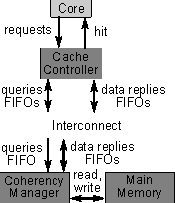
\includegraphics[width=14em]{\chapterdirectory/../cache_coherence/figure/cmp_overview.pdf}
\caption{Overview}%
\label{fr:fig:cache-coherence-cmps-overview}
\end{subfigure} &
\begin{subfigure}[t]{0.47\textwidth}
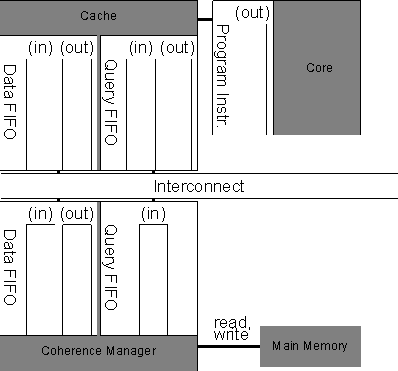
\includegraphics[width=20em]{\chapterdirectory/../cache_coherence/figure/cmp_detailed.pdf}
\caption{Showcasing the FIFOs}%
\label{fr:fig:cache-coherence-cmps-fifos}
\end{subfigure}
\end{tabular}
\end{center}
\caption{Components involved in cache coherence}%
\label{fr:fig:cache-coherence-cmps}
\end{figure}

\todomsg{Translate the figures in Figure~\ref{fr:fig:cache-coherence-cmps}}

\paragraph{\'El\'ement m\'emoire :}~~\\
The memory of a system is partitioned into addressable blocks. That is, there
are blocks of a certain size for which performing any access operation on its
content requires performing an operation on the block in its entirety.
To avoid unwarranted complications, this thesis considers that memory elements
are cache lines with the size of a single addressable block, making them atomic
blocks. The term memory element is used instead of cache line so that this
simplification remains explicit. Furthermore, since there is
only a single address per memory element, a memory element and its address can
be used interchangeably to refer to one another.

\begin{definition}[Memory Element]
\label{fr:def:memoryelement}
The set of all memory elements is defined as $\memoryelements{} \subseteq
\mathbb{N}$.
\end{definition}

\paragraph{C\oe{}ur et programme :}~~\\
Cache coherence is only affected by programs accessing the memory. As a result,
only the instructions related to the writing (\storeinstr{}), reading
(\loadinstr{}), and the eviction (\evictinstr{}) of memory elements are of any
considered while examining cache coherence. All other instructions are
assimilated into the no operation instruction (\nopinstr{}).

\begin{definition}[Instruction]
The set of all operators is defined as $\operators{} = \{\loadinstr{},
\storeinstr{}, \evictinstr{}, \nopinstr{}\}$, and instructions are defined
as $\instructions{} = \operators{} \times \memoryelements{}$
\end{definition}

\begin{definition}[Program]
Programs are sequences of instructions, thus $\programs{} =
\sequenceof{\instructions{}}$.
\end{definition}

\paragraph{Cache :}~~\\
\begin{definition}[Cache]
\label{fr:def:cache}
The set of all caches in the system is defined as \caches{}.  Some components
are present in both the caches and the coherence manager. We define
$\cachesandcmgr{} = \caches{} \cup \{\cmgr{}\}$ to add the coherence manager
(\cmgr{}). Furthermore, we define \nocache{}, not included in \caches{}, to
indicate the absence of a cache where one could be. The caches can also be
referred to using naturals from $1$ to \cachecount{}, with
$\cachecount{} = |\caches{}| - 1$.
\end{definition}

Caches are tasked with obtaining copies of memory elements able to fulfill the
memory accesses that are requested of them by their core. This requires keeping
track of permission for each copy of memory element they own, as well as
keeping track of operations (steps of the resolution of an instruction) that
are in progress. To do so, all caches assign a single state to each of their
memory element copies. These states are split into two categories:
\textit{stable} states, solely denoting that the cache has a certain permission
for that memory element, and \textit{transient} states, which indicate that the
resolution of a core's request is in progress and still awaiting either the
broadcast of a previously prepared query, or the reception of a data message
(or both).

To acquire new permissions, caches send queries on the interconnect. Each of
these queries pertains to a single memory element and leads to at most a single
reply being received by the emitter. For most types of data replies, a copy of
the memory element is part of the message. The types of queries that can be
sent are dependent on the actual cache coherence protocol. However, the
protocols used in this thesis all rely on the same ones: demand a read-only
copy of a memory element (\getsquery, likely following a \loadinstr{}
instruction), demand a read-and-write copy (\getmquery, likely following a
\storeinstr{} instruction), and signal the eviction of a potentially modified
copy (\putmquery, likely following an \evictinstr{}). Similarly, the
types of replies that can be exchanged are also dependent on the coherence
protocol. For those described in this thesis, only three types are required: a
message containing the memory element (\simpledata), one also indicating that
no other cache currently has access to that memory element (\exclusivedata),
and a message indicating that no copy of the memory element is going to be sent
(\nodata).

\begin{definition}[Query]
The categories of queries are defined as $\queries{} = \{\getsquery,
\getmquery, \putmquery\}$. A query message is an element of
$\querymessages{}: \queries{} \times \memoryelements{} \times \caches$, which
indicates the type of query, the memory element being targeted, and the
query's emitter.
\end{definition}

\begin{definition}[Reply]
The categories of reply messages are defined as $\replies{} = \{\simpledata,
\allowbreak{}
\exclusivedata,\allowbreak{} \nodata\}$. A reply message is an element of $\replymessages{}:
\replies{} \times \memoryelements{} \times \cachesandcmgr{}$, which indicates
its category, relevant memory element, and targeted cache (or \cmgr{}, when
targeting the coherence manager).
\end{definition}

Depending on what the cache coherence protocol allows, it is possible for
caches to receive queries they are in charge of replying to, despite not yet
having the data to do so. To handle such cases, caches can associate the
identifier of another cache with each address.

\begin{definition}[Information in Caches]
\label{fr:def:cache_info}
Each cache associates a state to each memory element, and can also associate
with it the identifier of another cache. We define $\cachestatefun{} :
\caches{} \to \memoryelements{} \to \cachestate{}$ as the function indicating
the state associated with a given memory element by a given cache, and
$\replytofun{} : \caches{} \to \memoryelements{} \to (\caches{} \cup
\{\nocache{}\})$ is the function indicating the cache (or lack thereof)
expecting a data reply in the future for a given memory element in a given
cache.
\end{definition}

Each cache has four FIFO queues, each one handling either incoming or outgoing
queries or data messages, as seen in
Figure~\ref{fr:fig:cache-coherence-cmps-fifos}.

\begin{definition}[Cache FIFOs]
\label{fr:def:cache_fifos}
The four FIFOs of each cache are defined as:
$\cachedatainfun{} : \cachesandcmgr{} \to \sequenceof{\replymessages{}}$ and
$\cachedataoutfun{} : \cachesandcmgr{} \to \sequenceof{\replymessages{}}$ for the
incoming and outgoing data message queues;
$\cachequeryinfun{} : \cachesandcmgr{} \to \sequenceof{\querymessages{}}$ and
$\cachequeryoutfun{} : \caches{} \to \sequenceof{\querymessages{}}$ for the
incoming and outgoing query message queues.
\end{definition}

\paragraph{Gestionnaire de coh\'erence :}~~\\
Maintaining cache coherence requires the caches to coordinate with each other.
Depending on the protocol, this may require some information to be accessible
to all caches. The coherence manager is a representation of this information.
This may not match any single one physical component of the system.
he role of the coherence manager is to act when none of the caches is
able to provide an answer to a cache's query. In order to detect such queries,
the coherence manager also assigns a state to each memory element.

\begin{definition}[Coherence Manager]
\label{fr:def:cmgr_info}
Let \coherencemanagerstate{} the set of states that can be attributed by the
coherence manager, $\coherencemanagerstatefun{} : \memoryelements{} \to
\coherencemanagerstate{}$ is the function indicating which state is attributed
to each memory element. The cache (or lack thereof) associated with each memory
element is defined as $\coherencemanagerownerfun{} : \memoryelements{} \to
(\caches{} \cup \{\nocache{}\})$.
\end{definition}

Much like the caches, the coherence manager uses FIFO queues to handle incoming
and outgoing messages. It has one less queue however, as the coherence manager
never sends any query. This can be seen in Definition~\ref{fr:def:cache_fifos},
where all but one of the types of FIFO queues are shared with the caches.

\paragraph{Interconnect:}~~\\
The interconnect links all caches together, as well as the coherence manager.
It broadcasts queries from the caches to all the components it is linked to,
including the original query emitter. The replies, however, are targeted, and
thus only received by a single component.

A system maintaining cache coherence is a system in which the application of
each read and write instruction on the same memory elements across multiple
caches holds the same results as if these caches shared a permanent single copy
of each of those memory elements.

\subsubsection{Les principes de la coh\'erence}
One possible strategy to achieve cache coherence is to enforce
Properties~\ref{fr:prop:system_wide_value}, \ref{fr:prop:swmr}, and
\ref{fr:prop:forget_me_not}. Other approaches may also be possible, but this is
the one considered in this thesis.

\begin{property}[Caches Have the System-Wide Value]%
\label{fr:prop:system_wide_value}
At any point, for each memory element, all copies of that memory element being
held in a cache have the value that was last written to that memory element,
regardless of which cache performed the writing.
\end{property}

\begin{property}[Single Writer or Multiple Readers]%
\label{fr:prop:swmr}
At any point, for each memory element, there is either a single cache being
able to write to that memory element while the others can neither read nor
write to it, or there is any number of caches being able to read the memory
element and none able to write to it.
\end{property}

\begin{property}[Forget Me Not]%
\label{fr:prop:forget_me_not}
If a memory element has no copy held in cache, then the system's main memory
has the value that was last written to that memory element.
\end{property}

\subsubsection{Aper\c{c}u du protocole MSI}
\label{fr:sec:intro_to_msi}
The archetypal cache coherence protocols are those belonging to the MSI
protocol family. In their basic version, these protocols feature three stable
states from which the MSI name is derived:
\begin{itemize}
\item \textbf{Modified:}
When a cache assigns the Modified state to a memory element, it indicates that
this cache performed at least one write to that memory element. While in this
state, it can freely read and write to that memory element. This corresponds
to being the \textit{Single Writer} from Property~\ref{fr:prop:swmr}.

\item \textbf{Shared:}
When a cache assigns the Shared state to a memory element, it indicates that
this cache is able to freely read that memory element but not write to it. This
corresponds to being one of the \textit{Multiple Readers} (and potentially the
only one) of Property~\ref{fr:prop:swmr}.

\item \textbf{Invalid:}
When a cache assigns the Invalid state to a memory element, it is no longer
considered to be holding a copy of that memory element, thus absolving this
cache from verifying Property~\ref{fr:prop:system_wide_value}. Not having a copy,
the cache can neither read nor write to the memory element.
\end{itemize}

\stopallthesefloats
\begin{figure}
   \begin{center}
   \begin{subfigure}[b]{0.7\linewidth}
      \begin{tikzpicture}[->,>=stealth',shorten >=1pt,auto,node distance=5cm,
                    semithick]
   \node[state] (I)              {\texttt{I}};
   \node[state] (S) [right of=I] {\texttt{S}};
   \node[state] (M) [below of=I] {\texttt{M}};

   \path[every node/.style={}]
      (I) edge [bend left] node {\textcolor{blue}{\loadinstr{}}?\textcolor{red}{\textcolor{red}{\getsquery{}}}!\textcolor{OliveGreen}{\simpledata{}}?} (S)
      (I) edge [bend right, sloped, anchor=center] node[yshift=-1em] {\textcolor{blue}{\storeinstr{}}?\textcolor{red}{\textcolor{red}{\getmquery{}}}!\textcolor{OliveGreen}{\simpledata{}}?} (M)

      (S) edge node {\textcolor{blue}{\evictinstr{}}?} (I)
      (S) edge [bend right=90, above] node {\textcolor{red}{\textcolor{red}{\getmquery{}}}?} (I)
      (S) edge [bend left, sloped, anchor=center] node[yshift=1.5em] {\textcolor{blue}{\storeinstr{}}?\textcolor{red}{\textcolor{red}{\getmquery{}}}!\textcolor{OliveGreen}{\simpledata{}}?} (M)
      (S) edge [out=430,in=400,looseness=8] node {\textcolor{blue}{\loadinstr{}}?} (S)

      (M) edge [bend left=90, above, sloped] node {\textcolor{red}{\textcolor{red}{\getmquery{}}}?\textcolor{OliveGreen}{\simpledata{}}!} (I)
      (M) edge [bend right=90, above, sloped, anchor=center] node[yshift=-1em] {\textcolor{red}{\textcolor{red}{\getsquery{}}}?\textcolor{OliveGreen}{\simpledata{}}!\textcolor{OliveGreen}{\simpledata{}}!} (S)
      (M) edge [sloped, anchor=center] node[yshift=-1em]
         {\textcolor{blue}{\evictinstr{}}?\textcolor{red}{\putmquery{}}!\textcolor{OliveGreen}{\simpledata{}}!} (I)
      (M) edge [out=230,in=200,looseness=8] node {\textcolor{blue}{\loadinstr{}}?} (M)
      (M) edge [out=280,in=250,looseness=8] node {\textcolor{blue}{\storeinstr{}}?} (M)
   ;
\end{tikzpicture}

      \caption{Cache}
      \label{fr:fig:general_msi_cc}
   \end{subfigure}
   \\
   \begin{subfigure}[b]{0.5\linewidth}
      \begin{tikzpicture}[->,>=stealth',shorten >=1pt,auto,node distance=5cm,
                    semithick]
   \node[state] (U)              {\texttt{I}};
   \node[state] (M) [left of=U] {\texttt{M}};

   \path[every node/.style={sloped, anchor=center, yshift=1em}]
      (U) edge [bend left] node {\textcolor{red}{\textcolor{red}{\getmquery{}}}?\textcolor{OliveGreen}{\simpledata{}}!} (M)
      (U) edge [loop below] node [below,yshift=-1em] {\textcolor{red}{\textcolor{red}{\getsquery{}}}?\textcolor{OliveGreen}{\simpledata{}}!} (U)

      (M) edge [bend left] node {\textcolor{red}{\putmquery{}}?\textcolor{OliveGreen}{\simpledata{}}?} (U)
      (M) edge [bend left=90] node {\textcolor{red}{\textcolor{red}{\getsquery{}}}?\textcolor{OliveGreen}{\simpledata{}}?} (U)
   ;
\end{tikzpicture}

      \caption{Coherence Manager}
      \label{fr:fig:general_msi_cmgr}
   \end{subfigure}
   \begin{subfigure}[b]{0.3\linewidth}
      \begin{tikzpicture}[->,>=stealth',shorten >=1pt,auto,node distance=5cm,
                    semithick]
   \node[state] (U)              {};

   \path[every node/.style={sloped, anchor=center, yshift=1em}]
      (U) edge [loop left] node [below,yshift=0.5em] {\textcolor{blue}{\loadinstr{}}!} (U)
      (U) edge [loop right] node [below,yshift=-1em] {\textcolor{blue}{\storeinstr{}}!} (U)
      (U) edge [loop below] node [below,yshift=-1em] {\textcolor{blue}{\evictinstr{}}!} (U)
   ;
\end{tikzpicture}

      \caption{Core}
      \label{fr:fig:general_msi_cpu}
   \end{subfigure}
   \end{center}
   \caption{Overview of the MSI Protocol}
   \label{fr:fig:general_msi}
\end{figure}

To keep it simple, the protocol presented in this section does not use any FIFO
queue. Instead, all exchanges are done synchronously. The only elements taken
into account are the state of the memory elements and the points of
synchronization (i.e. instruction and message exchanges). Thus, the notations
are not those presented in the previous section, but instead based on CCS
(Calculus of Communicating Systems, \cite{10.5555/539036}): a \texttt{?} marks
the reception of a signal, and \texttt{!} marks its sending.  Queries are still
sent to all components, and data only to a single one.  Furthermore, only a
single transaction (that is, the resolution of an instruction) can occur at any
moment. This is reflected by transitions featuring multiple synchronizations,
as no other actions would be permitted to be interleaved.

Figure~\ref{fr:fig:general_msi} shows the two automata corresponding to this
simplified protocol. Each of these automata pertains to a single memory element,
with states corresponding to what the component attributes to that memory
element.

In the case of the coherence manager (Figure~\ref{fr:fig:general_msi_cmgr}), the
two states simply correspond to whether or not the coherence manager is in
charge of providing the current value for that memory element: \texttt{M}
indicates that one of the caches is currently in the \texttt{M} state, meaning
that the value stored in the system's main memory may be out of date; \texttt{I}
indicates that the main memory's value for that element is up-to-date, leaving
(in the MSI protocol) the coherence manager in charge of propagating copies
as the caches demand them.

\begin{example}%
\label{fr:ex:general_msi_single_store}
Consider a system with two caches, $C_A$ and $C_B$, and a single memory
element $E$, such that, initially, $C_A$ holds no copy of $E$ (\texttt{I}
state) and $C_B$ holds one in the \texttt{S} state, the coherence manager
has the \texttt{I} state assigned to $E$. Were $C_A$ to receive a \storeinstr{}
request, it would broadcast a \getmquery{} to itself, $C_B$, and the coherence
manager. Upon receiving the \getmquery{}, $C_B$ would have to abandon the
\texttt{S} state for \texttt{I} in order to maintain Property~\ref{fr:prop:swmr}.
The coherence manager would react to receiving the \getmquery{} by sending a
copy of $E$ from the system's main memory to $C_A$ (\simpledata!)
before moving to \texttt{M} so as to memorize that the most up-to-date value
for $E$ is now held by $C_A$. This \simpledata{} reply allows $C_A$ to move to
the \texttt{M} state, thus completing its transition.
\end{example}

\todomsg{Add paragraph about how the real protocols are more complex}
